\section{Concepts and Background}\label{sec:backgroundML}
Machine learning refers to a set of techniques for understanding data. The theoretical subject of ``learning'' is related to prediction. Machine learning techniques involve building a statistical model for predicting, or estimating an output based on one or more inputs. Regression models are used when the output is a continuous value. In this work, we used three different machine learning methods: Linear Regression, Support Vector Machines and Random Forest. There exists other machine learning techniques with sophisticated learning process. However, in this work, we wanted to use simple models to prove that they achieve reasonable predictions.

\subsection{Linear Regression (LR)}
Linear regression is a straightforward technique for predicting a quantitative response $Y$ on the basis of a single or multiple predictor variables $X_p$. It assumes that there is approximately a linear relationship between each $X_p$ and $Y$. It gives to each predictor a separate slope coefficient in a single model. Mathematically, we can write the multiple linear regression model as
\begin{equation}
Y \approx \beta_0 + \beta_1 X_1 + + \beta_2 X_2 + \ldots + + \beta_p X_p + \epsilon
\end{equation}
where $X_p$ represents the $p$th predictor and $\beta_p$ quantifies the association between that variable and the response.

\subsection{Support Vector Machines (SVM)}
Support Vector Machines is a widely used technique for classification and regression problems. It belongs to the general category of kernel methods, which are algorithms that depend on the data only through dot-products. The dot product can be replaced by a kernel function which computes a dot product in some possibly high dimensional feature space $Z$. It maps the input vector $x$ into the feature space $Z$ though some nonlinear mapping. 

\subsection{Random Forest (RF)}
Random Forests belong to decision tree methods, capable of performing both regression and classification tasks. In general, a decision tree with $M$ leaves divides the feature space into $M$ regions $R_m$, $1 \leq m \leq M$. The prediction function of a tree is then defined as $f(x) = \sum_{m=1}^{M} c_m I(x, R_m)$, where $M$ is the number of leaves in the tree, $R_m$ is a region in the features space, $c_m$ is a constant corresponding to region $m$ and $I$ is the indicator function, which is 1 if $x \in R_m$, 0 otherwise. The values of $c_m$ are determined in the training process. Random forest consists of an ensemble of decision trees and uses the mode of the decisions of individual trees.

\subsection{Extraction Features Techniques}\label{ssec:ML}

Correlation techniques and hierarchical clustering algorithm were used in the phase of extraction features to reduce dimensionality of the features. Here, we show a short theoretical background of the techniques used in this work. 

There exist different correlation functions, among them, Pearson, Spearman and Kendal. The Pearson's correlation evaluates the linear relationship between two continuous variables, but omit variation in different scales. The Spearman's correlation evaluates the monotonic relationship between two continuous or ordinal variables. Besides Spearman correlation consider relations in different scales and spaces of the features due to the rank variables.

Pearson's correlation is commonly represented by the greek letter ($\rho$) when it is used for populations and by the letter $r$ when it is used for samples. We will denote it with the letter $r$, the formula for $r$ in a simplified form is
\begin{equation}
r=\frac{\text{cov}(X,Y)}{\sigma_{X}\sigma_{Y}},
\end{equation}
where, cov($X,Y$) is the covariance between two variables, $X$ and $Y$, $\sigma_{X}$ is the standard deviation of $X$ and $\sigma _{Y}$ is the standard deviation of $Y$.

The Spearman correlation coefficient is defined as the Pearson correlation coefficient between the ranked variables~\citep{myers2010research}, for a sample of size $n$, the $n$ raw scores $X_{i}$, $Y_{i}$ are converted to ranks rg$X_{i}$ rg$Y_{i}$. Here, this correlation is denoted as $r_s$, the formula for $r_s$ in a short manner is
\begin{equation}
r_{s}=\frac{\text{cov}(rgX,rgY)}{\sigma_{rgX}\sigma_{rgY}},
\end{equation}
where cov($rgX,rgY$) is the covariance of the rank variables, and $\sigma_{rgX}$ and $\sigma_{rgY}$ are the standard deviations of the rank variables. 

Hierarchical clustering creates groups from a distance matrix. Different metrics or distance functions exist in the literature, among them, Euclidean, Manhattan, Canberra, Binary or Minkowski, however, correlation functions can be also used. A heatmap of pair-wise correlations is a simple way to discover relationships between  pairs of quantitative variables in a dataset. A dendrogram is a tree diagram frequently used to illustrate the arrangement of the clusters produced by a hierarchical clustering algorithm. In Figure \ref{fig:heatMaphClust} is shown a dendrogram with its respective distance matrix using a Spearman correlation function. We can see in this figure a dendrogram with 10 different features about the profile information. In this figure red cells have a high correlation while blue cells have a low correlation.

\begin{figure}[htpb]
    \centering
    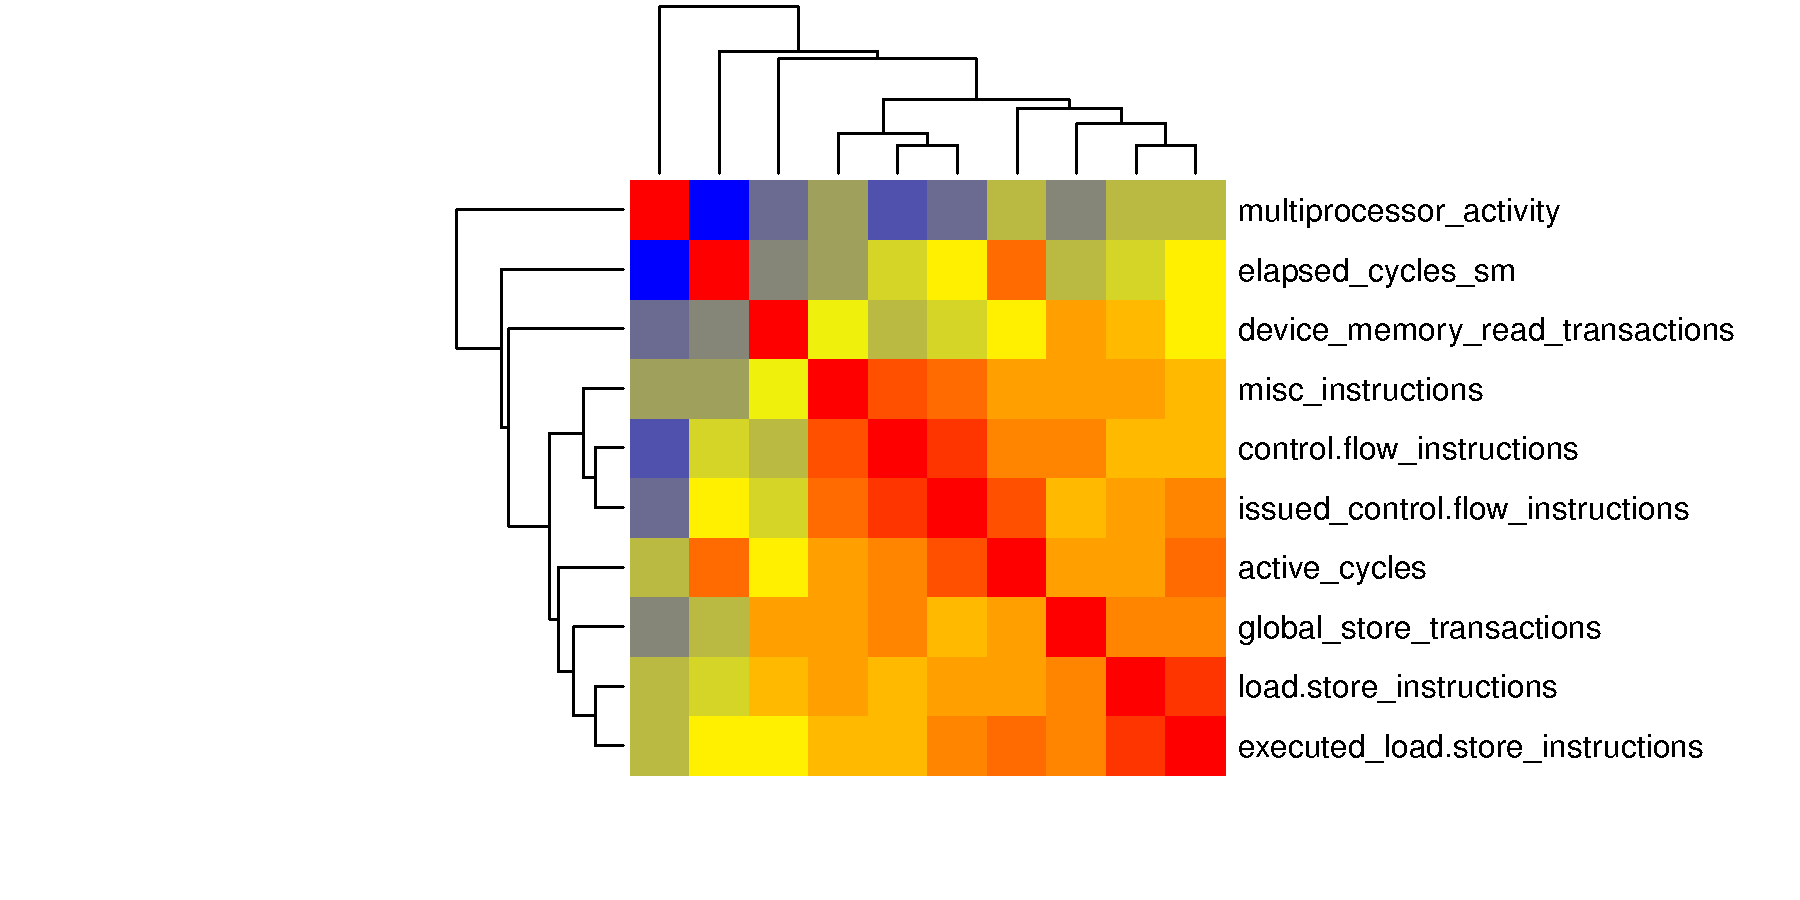
\includegraphics[scale=.5]{./images/heatMap.pdf}
    \caption{Heatmap and Dendrogram of a correlation matrix with some features in the experiments}
    \label{fig:heatMaphClust}
\end{figure}

A dendrogram is a tree diagram frequently used to illustrate the arrangement of the clusters produced by hierarchical clustering algorithms. In Figure \ref{fig:heatMaphClust} is shown a dendrogram with its respective matrix of correlation. This dendrogram can be cut in a certain height to permit create a specific number of clusters.